\chapter{Testing and Evaluation}
\label{chap:Testing and Evaluation}

\section{Unit Tests}
\label{sec:Unit Tests}

As mentioned in Section~\ref{sec:GoLang}, Go was originally designed to be a
modern alternative to C++. One of the major issues the original designers had
with C++, was the reliance on community tools\footnote{debuggers, profilers,
test libraries etc.} - some of which were high-quality, and many of which were
not. As a result, when developing GoLang, they wanted all the requisite tooling
to be built into the language, and authored by the language creators themselves,
to ensure a certain quality. As such, Go has support for unit tests out of the
box, without the need to consume third party libraries (more on that in
Section~\ref{sub:asyncTesting}). Tests can be invoked using \mintinline{bash}{go
test ./...}\footnote{Runs all unit tests in the current project}, which will
look for any files ending in \emph{\_test.go}, and run the tests they contain.
Tests belong to the same package as the software under test - meaning they
optionally have access to all private methods and variables, and can perform
black-and-whitebox testing. Files ending in \emph{\_test.go} are excluded from
standard compilation, however - so tests do not end up in the final compiled
binary.

An example of a test in Go is shown in (Listing~\ref{lst:goTest}). A test
function is simply one which begins with the word \emph{Test}, and which takes
in a test controller (\emph{t} in the given example). The test then performs
some actions (in this case, calling a method on the ConnectionManager), and
optionally fails the test by calling the relevant method on the test controller
(\mintinline{go}{t.Fail()}). Note that whilst the example given in
Listing~\ref{lst:goTest} is a unit test, integration tests are written using the
same formula. The output from the full test suite can be seen in the appendix
(Section~\ref{chap:testOutput}), as well as viewed online
(Section~\ref{sub:TravisCI}).

\begin{listing}[htbp]
  \centering
  \RecustomVerbatimEnvironment{Verbatim}{BVerbatim}{}
  \inputminted[firstline=13,lastline=27]{go}{code/gamq/connectionmanager_test.go}
  \caption{Testing the gamq connectionmanager}
  \label{lst:goTest}
\end{listing}

\subsection{Asynchronous Testing}
\label{sub:asyncTesting}

Whilst the built in Go unit testing fulfils the needs of most projects, several
third-party libraries have been written to improve the experience of testing
asynchronous code (Section~\ref{sub:concurrencyparallelism}). Blocks of code
which use GoRoutines/GoChannels (Section~\ref{sub:golangConcurrency}) will
behave in a non-deterministic manner, which can make testing them challenging.
For example, the block of

\subsection{Benchmarks}
\label{sub:benchmarks}

As well as ensuring the correctness of the code checked in, monitoring changes
in performance for certain critical sections of code is also a concern, when
building a system where speed is required. In order to do this, the built-in
GoLang test framework's benchmark support was used\footnote{Details about which
can be found in the \href{https://golang.org/pkg/testing/}{testing package
documentation}} to record stable execution times for critical functions.

\begin{listing}
  \centering
  \begin{minted}{Go}
func BenchmarkMessageQueue_Push(t *testing.B) {
	underTest := NewMessageQueue()
	testString := "test"

	for i := 0; i < t.N; i++ {
		underTest.Push(&testString)
	}
}
  \end{minted}
  \caption{An example of a benchmark in Go}
  \label{lst:goBenchmark}
\end{listing}

For example, Listing~\ref{lst:goBenchmark} shows a benchmark function to
evaluate the execution time of the \mintinline{Go}{Push()} function for my
MessageQueue implementation. When run as part of the \gls{ci} build, the
following output (Listing~\ref{lst:goBenchmarkOutput}) is given for each
benchmark. These results can then be compared across run, with the (still to be
implemented) option of failing the build in the event that a major increase in
average execution time for certain methods is detected, when compared to the
previous build (in a similar) manner to my code coverage metrics.

\begin{listing}
  \centering
  \begin{minted}[frame=single, framesep=10pt]{Bash}
BenchmarkMessageQueue_Push-2 # Benchmark Name
5000000 # Number of times loop executed to get a stable average
239 ns/op # Average execution time across all runs
  \end{minted}
  \caption{Example benchmark output}
  \label{lst:goBenchmarkOutput}
\end{listing}


\subsection{TravisCI}
\label{sub:TravisCI}

\missingfigure{Travis.CI screenshot}

Despite the initial plan being to set up and self-host most of the \gls{ci}
infrastructure, it became clear after an initial trial that it would be far
easier for to ensure build repeatability/speed if a cloud-based CI service was
used (some of the reasons for which are detailed below). The popular and
excellent \href{https://travis-ci.org/}{Travis CI} was selected - which provides
a free tier for open-source projects like gamq. Setup was as simple as adding a
`.travis.yml` file to the project, and enabling the gamq GitHub repo for builds
on the Travis CI admin panel. The initial .travis.yml file can be seen in
Listing~\ref{lst:initialTravis}, and the latest version is available
\href{https://github.com/FireEater64/gamq/blob/master/.travis.yml}{on GitHub}.
There are a multitude of configurable options available\footnote{More
information on the contents of .travis.yml files can be found in their
\href{https://docs.travis-ci.com/}{excellent documentation}.}, but the initial
configuration in Listing~\ref{lst:initialTravis} consisted of only three:

\begin{listing}
  \centering
  \begin{minted}[frame=single,framesep=10pt]{YAML}
language: go

go:
  - 1.3
  - 1.4
  - tip

script: go test -v ./... -bench=.
  \end{minted}
  \caption{Initial .travis.yml}
  \label{lst:initialTravis}
\end{listing}

\begin{description}
  \item[Language] Defines the language of the project being built - in this case
  \href{https://golang.org/}{GoLang}. TravisCI builds (usually) take place
  inside \href{https://www.docker.com/what-docker}{Docker containers}, with the
  'language' section of configuration dictating which pre-built container is
  used for this particular build. In this case, a language value of 'go' will
  ensure that the build container contains all of the binaries and environment
  variables required for building and running GoLang projects.
  \item[Go] This section defines different versions of the go compiler the
  project is built using. When code is checked in - Travis will spin up a
  separate Docker container (Section~\ref{sub:dockerDesign}) for each version
  specified, and run your complete test suite inside each container in parallel.
  This feature is known as the
  '\href{https://docs.travis-ci.com/user/customizing-the-build/#Build-Matrix}{build
  matrix}', and is \emph{incredibly} useful for ensuring software consistency on
  multiple different compilers/runtimes (especially useful for interpreted
  languages such as Java), and is something which would be hard to replicate
  outside of a containerised build environment (i.e. if using a self-hosted
  \gls{ci} environment).
  \item[Script] Any custom commands to be run as part of the build. Travis
  contains\footnote{Pun intended} a standard build script for most languages
  (which are selected via the 'language' configuration detailed above), however
  builds invariably require additional scripts/commands to be run as well - some
  example use cases could be to run additional tests, or deploy build binaries
  to an artifact repository. In this case, the commands specified execute both
  the unit/integration test suite, and the benchmark suite
  (Section~\ref{sub:benchmarks}).
\end{description}

\subsection{Coveralls}
\label{sub:Coveralls}

\missingfigure{Coveralls screenshot}

One important (though not definitive) metric associated with unit/integration
tests is \emph{code coverage}, which is the total percentage of the code-base
that is executed when running unit tests. This is a useful metric to keep an eye
on, as it helps\footnote{Though doesn't always} indicate which sections of code
are susceptible to bugs as a result of not being tested. Go's built in test
runner is capable of producing code coverage reports during test runs, however I
chose to use an open source tool called
'\href{https://github.com/axw/gocov}{gocov}', as it allowed me to send the code
quality metrics produced my build to another online service,
\href{https://coveralls.io/}{coveralls}. The reasons behind doing this, rather
than relying on the build-in HTML report were:

\begin{description}
  \item[Visibility] Publishing my code quality metrics in an easily accessibly,
  publicly visible website (as well as the front page of my GitHub project),
  rather than hiding them away in build logs helps to 'keep me honest', as well
  as '\textit{\gls{gamify}}' the process of driving up coverage.
  \item[Monitoring] Coveralls allows me to set 'thresholds' for coverage
  metrics, and will fail the build if these are not adhered to. For example, my
  build will fail if the coverage of the checked in code is even 0.1\% less than
  that of the previous successful build.
\end{description}

The code quality metrics for my project are available
\href{https://coveralls.io/github/FireEater64/gamq?branch=master}{on Coveralls},
as well as being summarised in the
\href{https://github.com/FireEater64/gamq/blob/master/README.md}{README for my
project on GitHub}\(Figure~\ref{fig:readmeStatus} \).

\begin{figure}
  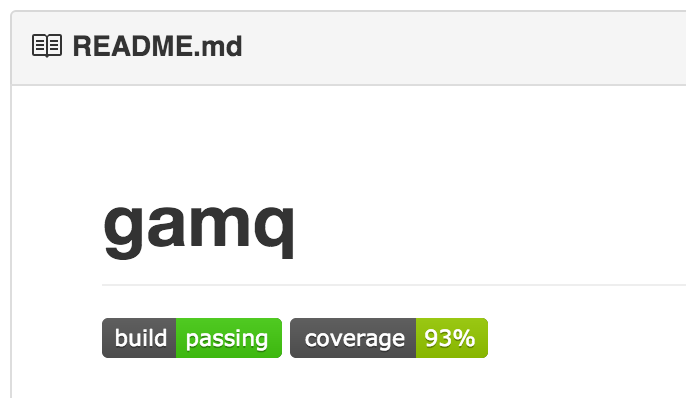
\includegraphics{figures/README}
  \centering
  \caption{Code status badges in README.md}
  \label{fig:readmeStatus}
\end{figure}

\section{Environmental Testing}
\label{sec:environmentalTesting}

In-place, or \emph{environmental} testing helps ensure that software/systems are
capable of full operation under sub-optimal circumstances. It is an important
step when writing software, as there are many design and implementation failings
that only become apparent under these suboptimal conditions. For example, a
message broker using UDP may appear to perform perfectly in a development
environment, but if the production environment spans multiple datacenters - the
high probability of packet loss on inter-datacenter links may cause problems.
This is one of the reasons development infrastructure should resemble that of
production as closely as possible, warts and all.

\subsection{Methodology}
\label{sub:Methodology}

\todo[inline]{Prof files/timings etc.}

\subsection{Tools}
\label{sub:Tools}

\todo[inline]{Network link conditioner/test scripts/presentation framework}

\section{System Performance}
\label{sec:System Performance}

\todo[inline]{Analysis of prof files/theoretical maximum limits/comparisons/potential improvements}
